\documentclass[11pt,oneside,letterpaper]{article}

% graphicx package, useful for including eps and pdf graphics
\usepackage{graphicx}
\DeclareGraphicsExtensions{.pdf,.png,.jpg}

% basic packages
\usepackage{color} 
\usepackage{parskip}
\usepackage{float}

% text layout
\usepackage{geometry}
\geometry{textwidth=15cm} % 15.25cm for single-space, 16.25cm for double-space
\geometry{textheight=22cm} % 22cm for single-space, 22.5cm for double-space

% helps to keep figures from being orphaned on a page by themselves
\renewcommand{\topfraction}{0.85}
\renewcommand{\textfraction}{0.1}

% bold the 'Figure #' in the caption and separate it with a period
% Captions will be left justified
\usepackage[labelfont=bf,labelsep=period,font=small]{caption}

% review layout with double-spacing
%\usepackage{setspace} 
%\doublespacing
%\captionsetup{labelfont=bf,labelsep=period,font=doublespacing}

% cite package, to clean up citations in the main text. Do not remove.
\usepackage{cite}
%\renewcommand\citeleft{(}
%\renewcommand\citeright{)}
%\renewcommand\citeform[1]{\textsl{#1}}

% Remove brackets from numbering in list of References
\renewcommand\refname{\large References}
\makeatletter
\renewcommand{\@biblabel}[1]{\quad#1.}
\makeatother

\usepackage{authblk}
\renewcommand\Authands{ \& }
\renewcommand\Authfont{\normalsize \bf}
\renewcommand\Affilfont{\small \normalfont}
\makeatletter
\renewcommand\AB@affilsepx{, \protect\Affilfont}
\makeatother

% comments
\usepackage{ulem}
\definecolor{purple}{rgb}{0.459,0.109,0.538}
\def\tb#1#2{\sout{#1} \textcolor{purple}{#2}} 
\def\tbc#1{\textcolor{purple}{[#1]}}



%%% TITLE %%%
\title{\vspace{1.0cm} \LARGE \bf Reassortment between influenza B lineages and the emergence of a co-adapted PB1-PB2-HA gene complex}

\author[1]{Gytis Dudas}
\author[2]{Trevor Bedford}
\author[1]{Samantha Lycett}
\author[1,3]{Andrew Rambaut}

\affil[1]{Institute of Evolutionary Biology, University of Edinburgh, Edinburgh, UK}
\affil[2]{Vaccine and Infectious Disease Division, Fred Hutchinson Cancer Research Center, Seattle, WA, USA}
\affil[3]{Fogarty International Center, National Institutes of Health, Bethesda, MD, USA}

\date{\today}

\begin{document}
\maketitle

\begin{abstract}

Influenza B viruses are increasingly being recognized as major contributors to morbidity attributed to seasonal influenza. 
Currently circulating influenza B isolates are known to belong to two antigenically distinct lineages referred to as B/Victoria and B/Yamagata lineages on the basis of haemagglutinin inhibition (HI) assays. 
Frequent reassortment between the segments of these two lineages has been noted in the past \cite{lindstrom1999}, but the effects of these reassortments have not been investigated in much detail.

\end{abstract}

\pagebreak

\section*{Introduction}
Seasonal influenza causes an estimated 250,000 to 500,000 deaths annually and is comprised of three virus types (A, B and C) co-circulating in humans, of which influenza A is considered to cause the majority of seasonal morbidity and mortality.
Though lacking the degree of antigenic diversity that influenza A viruses possess, influenza B viruses are increasingly being recognized as important human pathogens \cite{paul-glezen2013}.
Following the 2009 A/H1N1 pandemic, influenza B has increased in prevalence and in the 2012/2013 European season as many as 53\% of influenza sentinel surveillance samples tested positive for influenza B \cite{ECDC1213}. 

Like all members of \textit{Orthomyxoviridae}, influenza B viruses have segmented genomes, which allow viruses co-infecting the same cell to exchange segments (a process known as reassortment). 
Influenza A viruses are widely considered to be a major threat to human health worldwide due to the ability to cause pandemics in humans via reassortment of seasonal human and non-human influenza A strains. 
The only known persistent host of influenza B viruses are humans (and occasionaly seals \cite{osterhaus2000,bodewes2013}), thus limiting the virus's potential to exhibit pandemics through the acquisition of antigenic novelty from an animal reservoir. 
Both influenza A and B evolve antigenically through time in a process known as antigenic drift, in which mutations to the haemagglutinin (HA) protein allow viruses to escape existing human immunity and persist in the human population, leading to recurrent seasonal epidemics \cite{bedford2013}.

Currently circulating influenza B viruses are comprised of two distinct lineages -- Victoria and Yamagata (referred to as Vic and Yam, respectively) -- named after strains B/Victoria/02/87 and B/Yamagata/16/88, that are thought to have genetically diverged in HA around 1983 \cite{rota1990}. 
These two lineages possess antigenically distinct HA surface glycoproteins allowing them to co-circulate in the human population.
All other influenza B segments also show a split into two lineages around that time.

Previously, through the combined use of time-stamped and maximum likelihood phylogenetic trees evolutionary rate, selective pressures and reassortment history of major clades of influenza B have been analyzed \cite{chen2008}, showing extensive and often complicated patterns of reassortment between all segments of influenza B viruses both between and within Vic and Yam lineages.
This analysis was limited because it used limited and different numbers of sequences to infer trees of each segment and relied on maximum likelihood phylogenies to infer the history of reassortments.
Here, we introduce another approach that reveals a evolutionarily intriguing pattern of reassortment in influenza B.
In this approach, membership to either the Victoria or Yamagata lineage in the tree of one segment is used to label the individual viruses in the tree of the other segments.
Reassortment events which result in the replacement of one segment lineage by another show up as changes in the discrete trait along a branch (Figure \ref{methodFig}).
Here, we use discrete traits to reconstruct major reassortment events in the recent history of influenza B viruses and to partition diversity across segments of influenza B virus strains to quantify reassortment dynamics over time.

We show that despite extensive reassortment, PB1, PB2 and HA segments of influenza B viruses still survive as distinct Victoria (Vic) and Yamagata (Yam) lineages, which appear to be co-adapted to the point where virions which do not contain PB1, PB2 or HA segments derived entirely from either the Vic or the Yam lineage have rarely been isolated and once isolated belong to transient lineages.
In other segments (PA, NP, NA, MP and NS) a single lineage has been fixed in the influenza B population: Yam for PA, NP, NA and MP and Vic for NS.

\begin{figure}[h]
 \centering		
	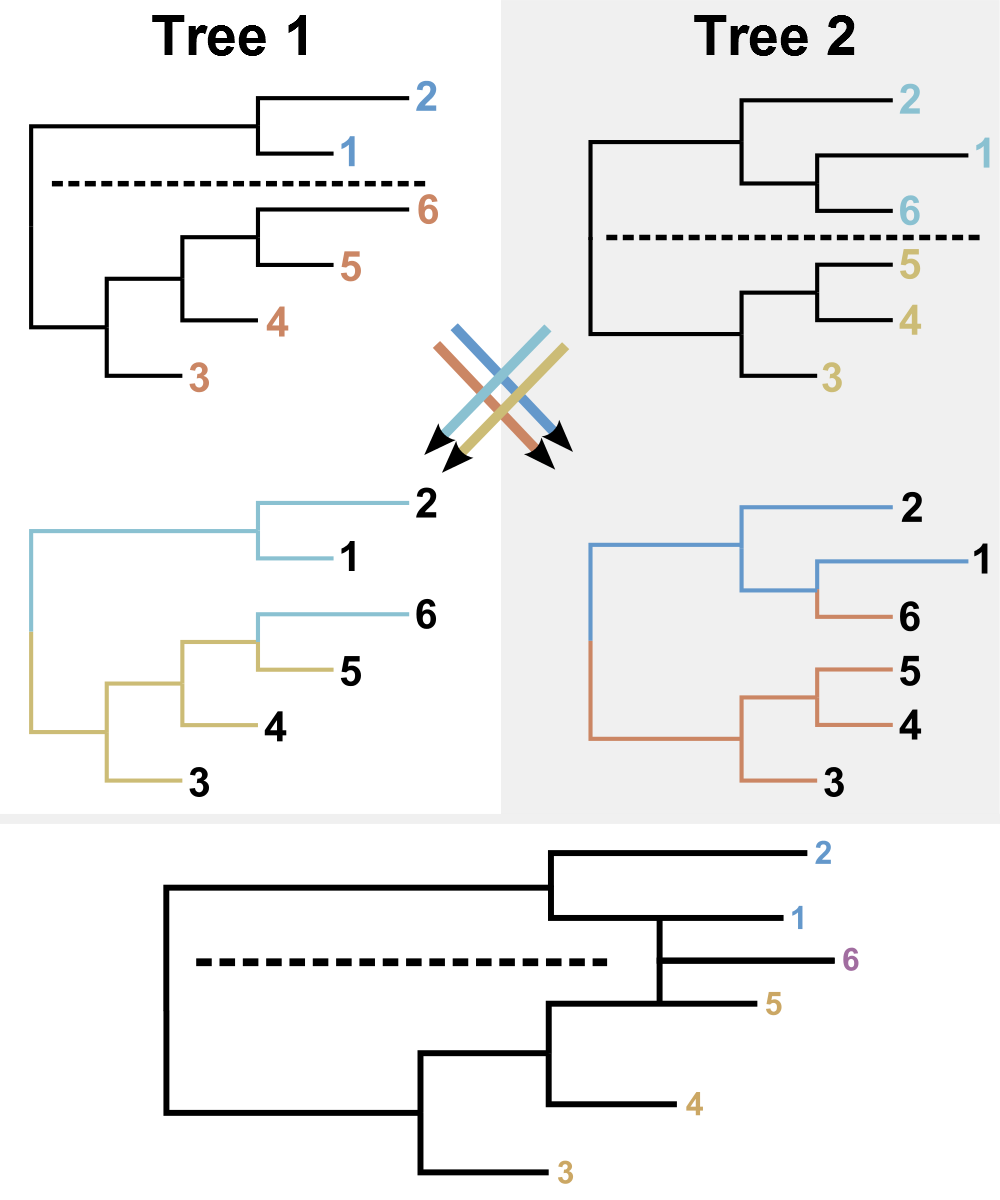
\includegraphics[width=0.45\textwidth]{figures/TreeFigure2}
	\caption{\textbf{Schematic depiction of method.}
We begin by assigning sequences falling on either side of a specified bifurcation within each segment tree to different lineages.
We then transfer lineage labels from one tree to the same tips in another tree.
Label switches thus indicate reassortment events that combine lineages falling on different sides of the bifurcation specified earlier.
In the example above tip number 6 is determined to be such a reassortant.}
	\label{methodFig}
\end{figure}

\section*{Methods}

\subsection*{Sequences and lineage assignment}

We compiled a dataset of 452 complete influenza B genomes from GISAID \cite{GISAID} dating from 1984 to 2012. 
Each strain was assigned to a lineage (either Vic or Yam) in each segment by making maximum likelihood trees and looking whether it fell within the subtree containing B/Victoria/02/87 or B/Yamagata/16/88 sequences with the exception of the NS segment (B/Victoria/02/87 was a reassortant and possessed a Yam lineage NS \cite{lindstrom1999}), where B/Czechoslovakia/69/1990 was considered as being representative of Victoria lineage.

Each strain was thus assigned 8 lineages depending on the combination of lineages it belongs to in all trees (for example all segments except for NS in strain B/Victoria/02/87 belong to Vic lineage and can thus be represented as V,V,V,V,V,V,V,Y). 

\subsection*{Building trees}
Temporally-calibrated phylogenies were recovered for each segment using the Markov chain Monte Carlo (MCMC) methods in the BEAST software package \cite{drummond2012}.
Here, we modeled the substitution process using the HKY model of nucleotide substitution, with separate HKY models for each of the 3 codon partitions, and additionally included robust counting \cite{obrien2009} to report realized substitutions.
We modeled the demographic process using a GMRF Bayesian skyride model \cite{minin2008}.
We used `relaxed' tips for 94 sequences (of which 93 only had year of isolation and 1 had only year and month of isolation) whereby tip date is estimated as a latent variable in the MCMC integration.
We ran 3 independent MCMC chains, each with 200 million states, sampled every 20000 steps and discarded the first 10\% of the MCMC states as burn-in.
Samples were combined across runs to give 27000 total samples for each segment and convergence was assessed by Tracer.

Every sequence was assigned 7 discrete traits corresponding to the lineages of all other segments with which a strain was isolated (e.g. PB1 tree had PB2, PA, HA, NP, NA, MP and NS as traits and V or Y as trait values).
We inferred the ancestral state of lineages in each segment by using discrete traits (asymmetric CTMC matrix with BSSVS \cite{lemey2009}). Because the posterior set of trees have branches labelled with the inferred lineage in all other segments, we can detect inter-lineage reassortments whenever a trait transition is observed (i.e. Yam to Vic or Vic to Yam, see Figure \ref{methodFig}) between a node and its descendant in any segment. 
In addition, by reconstructing the ancestral state of all other genomic segments jointly we can infer co-reassortment events when more than one trait transition occurs on the same node in a tree.

\subsection*{Measures of diversity}
We inferred the diversity of each segment over time by finding the most recent common ancestor of all branches existing at yearly intervals, which places an upper boundary on the maximum amount of diversity existing at each time period.
In addition, we calculated mean pairwise TMRCA between branches inferred to be in virions possessing Vic and Yam lineage PB1, PB2 and HA.
This gave us an averaged measure of how much a particular segment reassorts with respect to PB1, PB2 and HA segments.
If Vic and Yam lineages of PB1, PB2 and HA segments were to be considered as being separate populations this measure would be equivalent to `between population' diversity.

We also calculated the total amount of evolutionary time each segment has spent in virions with entirely Vic, entirely Yam or mixed lineage PB1, PB2 and HA segments by taking the sum of branch lengths in each tree under different combinations of the PB1, PB2 and HA labels.
This gives a measure of how successful, over long periods of time, each particular PB1-PB2-HA constellation has been.

\subsection*{Tree to tree similarities}
In order to get a measure of tree to tree similarity we first extracted 900 trees from the posterior distributions of trees for each segment.
These were combined across 3 independent MCMC chains to give a total of 2700 trees.
Pairwise comparison between each pair of segments was performed by comparing trees at each MCMC state.

We express the similarity of two trees by referring to the mean of the distribution of TMRCA differences ($\Delta$TMRCA) between pairs of tips in the two trees.
These parameters are estimated for each pairing of trees at each MCMC state and provides us with 95\% highest posterior density intervals for those parameters, thus giving us the ability to test specific hypotheses regarding similarities between the trees of different segments.
Our approach exploits the branch scaling used by BEAST \cite{drummond2012}, since the trees are scaled in absolute time and therefore insensitive to variation in nucleotide substitution rates between segments, allowing for direct comparisons between TMRCAs in different trees.

If we are comparing TMRCAs of the same two tips in tree A and tree B we express it as $\frac{[A:A']+[B:B']}{2\times [A:B]}$, where [A:B] is $\Delta$TMRCA of a pair of tips between tree A and tree B and [A:A'] is $\Delta$TMRCA between the same pair of tips between tree A and a replicate of tree A (A'), to control for variability in tree topology stability over the course of the MCMC chain caused by differences in alignment lengths used to produce the trees.

We also attempted to calculate subtree prune and regraft (SPR) distances between trees using rSPR \cite{whidden2009,whidden2010,whidden2013}.
However, because the time taken to calculate the SPR distances depends on the SPR distances themselves, we find that exact SPR distance calculations over posterior sets of trees are impractical for all but the most similar trees.
We thus calculated approximate SPR distances for all trees, using the normalization procedure described above.

\subsection*{Estimating linkage disequilibrium across the influenza B genome}
We attempted to estimate linkage disequilibrium (LD) between amino acid sites across the influenza B proteome.
We chose the $\chi^{2}_{df}$ statistic \cite{zhao2005} for quantifying LD, as it is equal to the widely used \textit{r$^{2}$} LD statistic at biallelic loci, but also quantifies LD when there are more than two alleles per locus.
LD was estimated only at loci where each `allele' was represented by at least two isolates and gaps were ignored and not considered as polymorphisms.
Ignoring gaps in estimating LD was a practical decision based on some sequences missing nucleotides at the beginning and end of sequences.
However, there is at least one polymorphic indel within the HA protein, which is associated with the Vic-Yam split and not with sequence quality.
In addition, some influenza B genome constellations have not reassorted for prolonged periods of time and have acquired amino acid substitutions on several segments, resulting in linkage disequilibrium.
These single site pairs result in high LD and come from poorly sampled lineages, thus we choose to only focus on alleles that have been sampled at least twice.

We also calculated mean LD for all pairs of segments to quantify associations between different segments.

\subsection*{Confirming findings with a larger dataset and lineage assignment to sequences}
The sequences of all 1433 available sequences of PB1, PB2, HA and NA segments from the same isolates were downloaded from GISAID.
Neighbour-joining trees of PB1, PB2 and HA segments were made and each sequence assigned to a lineage based on grouping with either B/Victoria/02/87 or B/Yamagata/16/88 sequences.
Isolates which were not assigned entirely to either the Vic or the Yam lineage across PB1, PB2 and HA segments were extracted and identified as PB1-PB2-HA reassortants.

\section*{Results}

\tbc{I think that for these first two sections, you just need figures \ref{tmrcaOT} and \ref{lineageRatiosOverTime}.  Figure \ref{betweenDiversity} seems redundant, and the multiple `perspectives' is confusing to be the first thing shown.}

\subsection*{PA, NP, NA, MP and NS segments have periodically lost diversity}

The split of Vic and Yam lineages can be seen in all segments \cite{chen2008}.
Following the split of the two lineages, each segment could be assigned to either Vic or Yam lineage and inter-lineage reassortment events have yielded mixed-lineage genome constellations.
Some viruses with mixed-lineage genomes have become common ancestors to many later strains (i.e. the `trunk' of the phylogenetic tree) and the segment lineages involved so successful, as to become fixed within the influenza B population circulating today.

We find that Vic lineage PA, NP, NA and MP segments have gone extinct (i.e. no sequences from those lineages have been sampled in recent years see Figure \ref{lineageRatiosOverTime}), replaced entirely by the respective segments of Yam lineage in viruses bearing a Vic lineage HA.
Similarly, Vic lineage NS has become fixed in the viral population as well.
By looking at the most recent common ancestor of all lineages existing at yearly timeslices within the tree of each segment (see Figure \ref{tmrcaOT}), it is clear that PA, NP, NA, MP and NS segments have undergone periodic losses of diversity, whereby all sequences sampled more recently trace their ancestry to increasingly more recent common ancestors.


\subsection*{PB1, PB2 and HA segments continue to circulate as two lineages and have not reassorted recently}
Unlike PA, NP, NA, MP and NS segments, which have periodically lost diversity, we find that PB1, PB2 and HA segments have continued to accumulate diversity since the initial split of Vic and Yam lineages (see Figure \ref{tmrcaOT}).
In addition, there is evidence to suggest that the numbers of sequences that belong to either Vic and Yam lineages of PB1, PB2 and HA segments have been sampled at a ratio close to 0.5 (see Figure \ref{lineageRatiosOverTime}), presumably due to the action of some form of balancing selection.

By measuring the mean pairwise diversity between branches in each tree that were assigned either a Vic or Yam label in other segments, we look for reductions in diversity, which indicate that an inter-lineage reassortment event has taken place and thus is a qualitative measure of panmixis between pairs of segments.

In Figure \ref{betweenDiversity} we focus on PB1, PB2 and HA lineage labels, which have both Vic and Yam lineages up to recent times.
We find that there have been some losses of diversity, indicative of label mixing i.e. reassortment, in the early years of the Vic--Yam split (1986--1996) between HA and PB1--PB2 segments.
After 1997, however, mean pairwise between label diversity increases in PB1, PB2 and HA segments, whereby Vic and Yam labels share a common ancestor only at the root.
Our data thus suggest that since 1997 there has been no reassortments between Vic and Yam lineages of PB1, PB2 and HA segments.
In addition mean pairwise between label diversity measurements after 1997 become identical regardless of chosen label, which suggests that PB1, PB2 and HA lineage labels are assigned identically in all trees investigated.

\begin{figure}[h]
	\centering		
	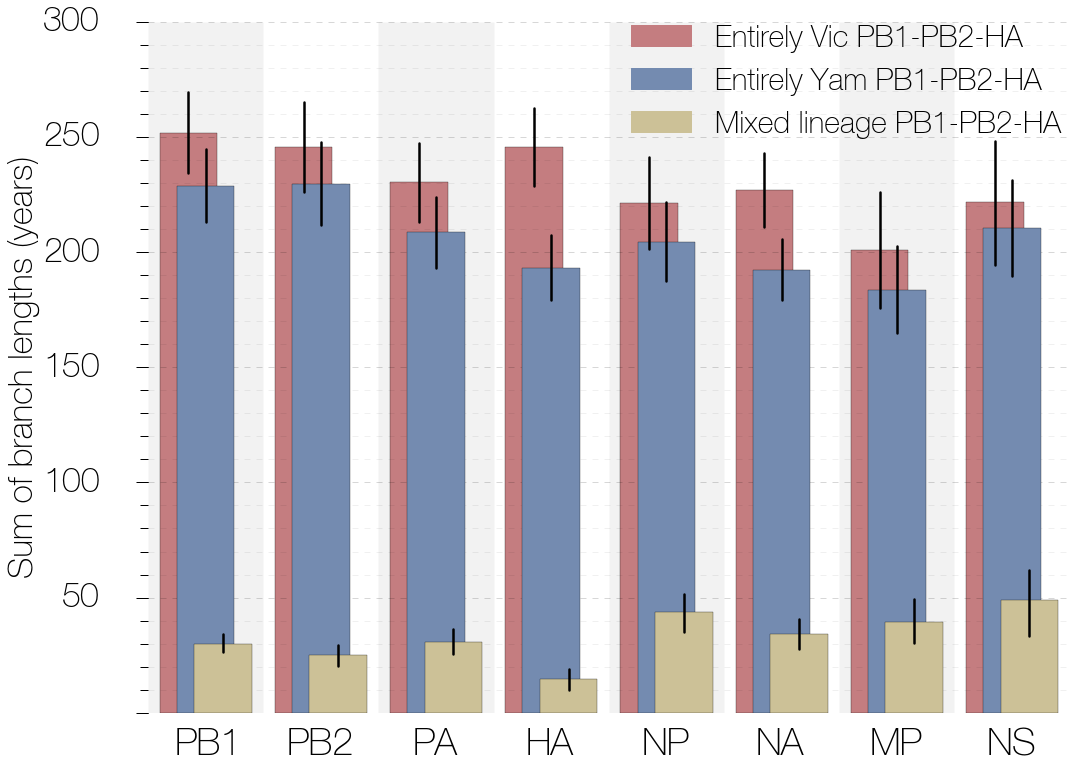
\includegraphics[width=0.95\textwidth]{figures/InfB_stateTime.png}
	\caption{\textbf{Amount of evolutionary time spent under different PB1-PB2-HA constellations.}
All segments have spent significantly more of their history with entirely Vic or entirely Yam-derived PB1-PB2-HA complexes.
All horizontal lines indicating uncertainty are 95\% highest posterior densities (HPDs).}
	\label{stateTime}
\end{figure}


\subsection*{Recent PB1-PB2-HA constellations are entirely derived from Victoria or Yamagata lineage segments}

\tbc{Did you decide to shelve the REPU statistics?  At least in theory, this should be much more convincing that PB1-PB2-HA are held together by selection rather than `mutation' (i.e. due to packaging signals).  REPU should be a stronger argument than figure \ref{betweenDiversity}. .... I see.  You can't do something like REPU if you don't observe any transient reassortants in the first place.  This suggests either that selection is very strong or mutation is very rare.  But later on you mention that `there have been at least 3 sampled mixed-lineage PB1-PB2-HA complex constellations'.  More description of these constellations would be helpful, when they appear and how long they last.  Also report how long the average lineage persists.}

\tbc{Can you reject the hypothesis that PB1 and PB2 stuck to HA stochastically?}

We find that PB1, PB2 and HA segments, in addition to not reassorting across the Vic-Yam lineage boundary recently, form co-reassorting segment complexes derived entirely of Vic or Yam lineage segments.
Figure \ref{stateTime} shows the sum of branch lengths which were labelled as having entirely Vic, entirely Yam or mixed-lineage PB1, PB2 and HA segments.
Due to lack of reassortment between Vic and Yam lineages of PB1, PB2 and HA (Figure \ref{betweenDiversity}) all segments have spent significantly longer periods of time with either entirely Vic-derived or entirely Yam-derived than with mixed-lineage PB1, PB2 and HA constellations.


We have identified 3 classes of mixed-lineage PB1-PB2-HA reassortants from our data with the following PB1-PB2-HA constellations: VVY (B/Bankok/163/1990-like, 13 sequences isolated 1990 -- 5th Jan 1995), YVV (B/Nanchang/630/1994-like, 2 sequences isolated 1994 -- 1996) and YVY (B/New York/24/1993-like, 2 sequences isolated 8th Jan 1993 -- 1994).
An additional class of reassortants with a YYV PB1-PB2-HA constellation (B/Waikato/6/2005-like, 16 sequences isolated June 9 -- November 12 in 2005) was found when investigating a larger dataset with only PB1, PB2, HA and NA sequences.
In all cases PB1-PB2-HA reassortants have not persisted for prolonged periods of time and have not been fixed in the influenza B population.
In particular reassortment events combining PB1 and PB2 segments of different lineages, e.g. B/Nanchang/630/1994-like and B/New York/24/1993-like isolates, exhibit poor sampling and short circulation times.
In contrast, reassortments combining PB1+2 and HA of different lineages (B/Bankok/163/1990-like and B/Waikato/6/2005-like isolates) have more isolates and circulated for much longer periods of time in the past.

\begin{figure}[h]
	\centering		
	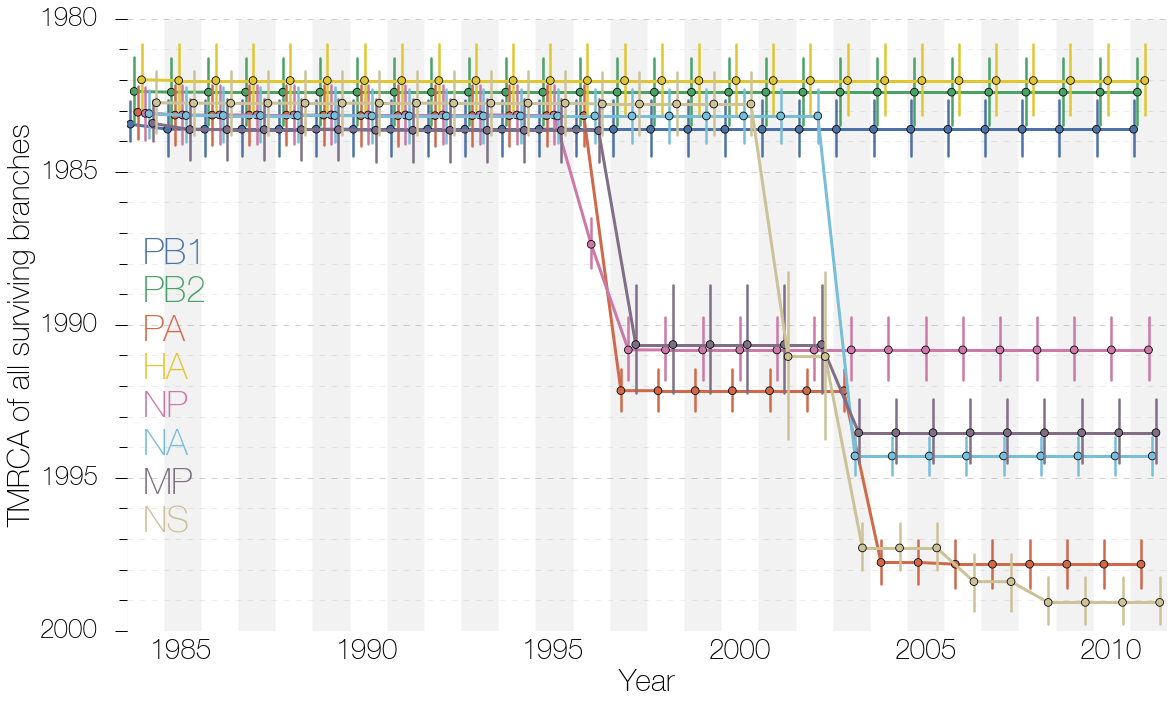
\includegraphics[width=0.95\textwidth]{figures/InfB_tmrcaOT_lines.png}
	\caption{\textbf{Oldest TMRCA of all surviving lineages over time.}
PA, NP, NA, MP and NS segments of influenza B viruses show periodic losses of diversity, indicating lineage turn over.
PB1, PB2 and HA segments, on the other hand, maintain the diversity dating back to the initial split of Vic and Yam lineages.
All vertical lines indicating uncertainty are 95\% highest posterior densities (HPDs).}
	\label{tmrcaOT}
\end{figure}

(comment - need higher resolution for lineage ratios figure or switch to vector graphics)
\begin{figure}[h]
	\centering	
	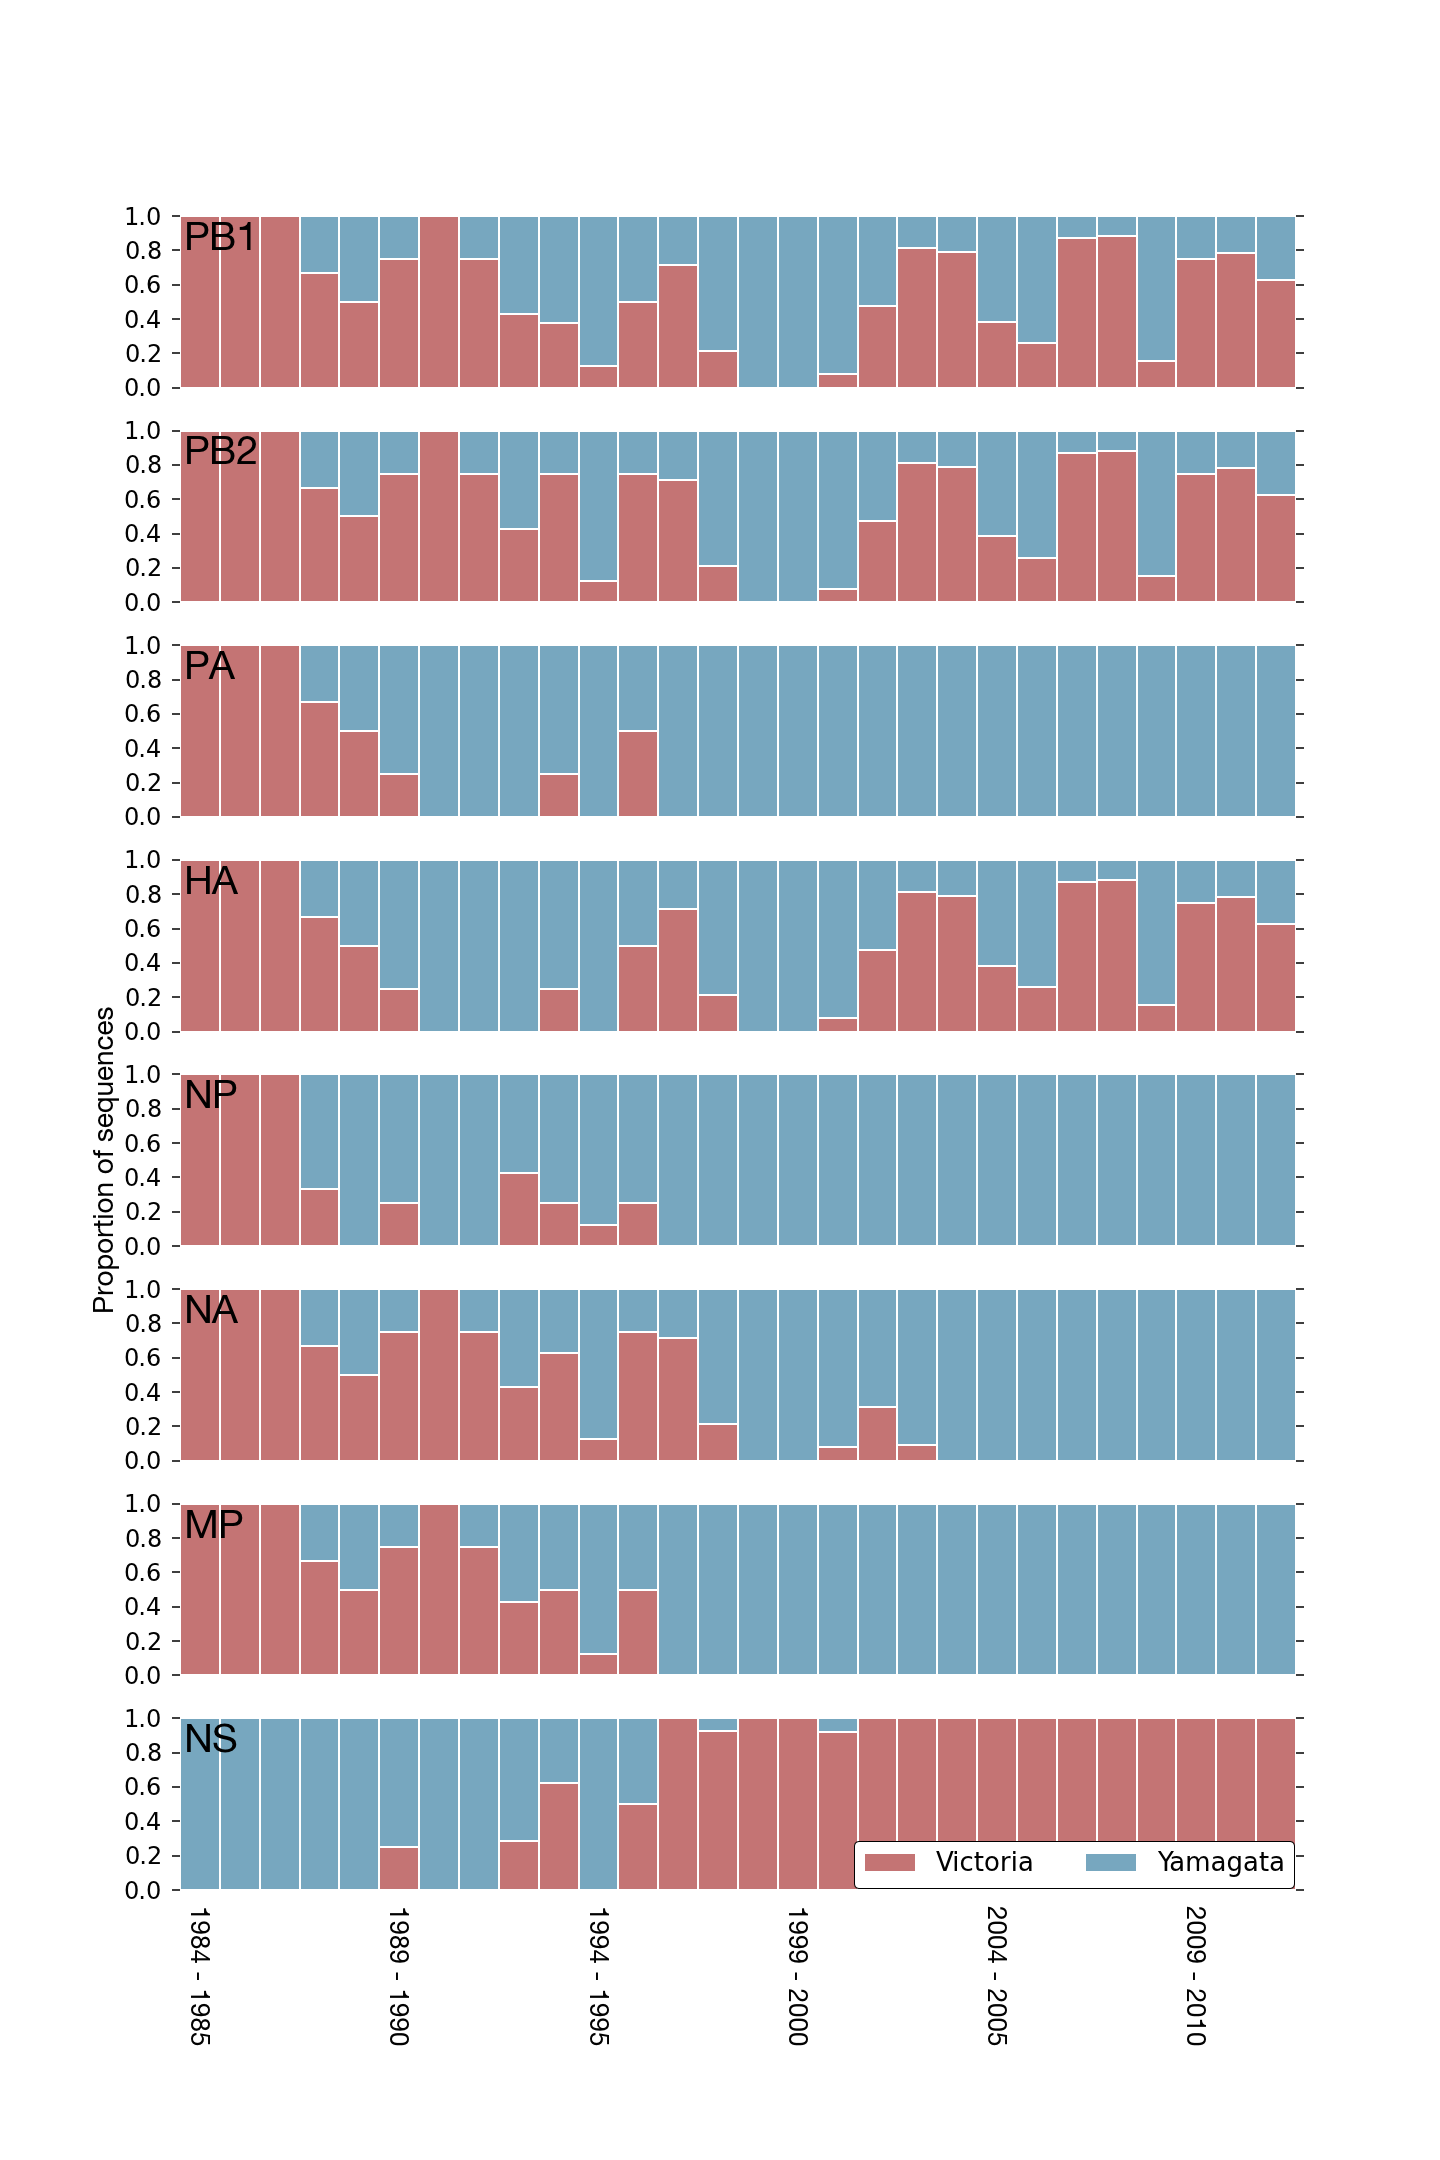
\includegraphics[width=0.75\textwidth]	{figures/InfB_LineageRatiosOverTime.png}
	\caption{\textbf{Ratio of lineages in the dataset.}}
	\label{lineageRatiosOverTime}
\end{figure}

\begin{figure}
	\centering		
	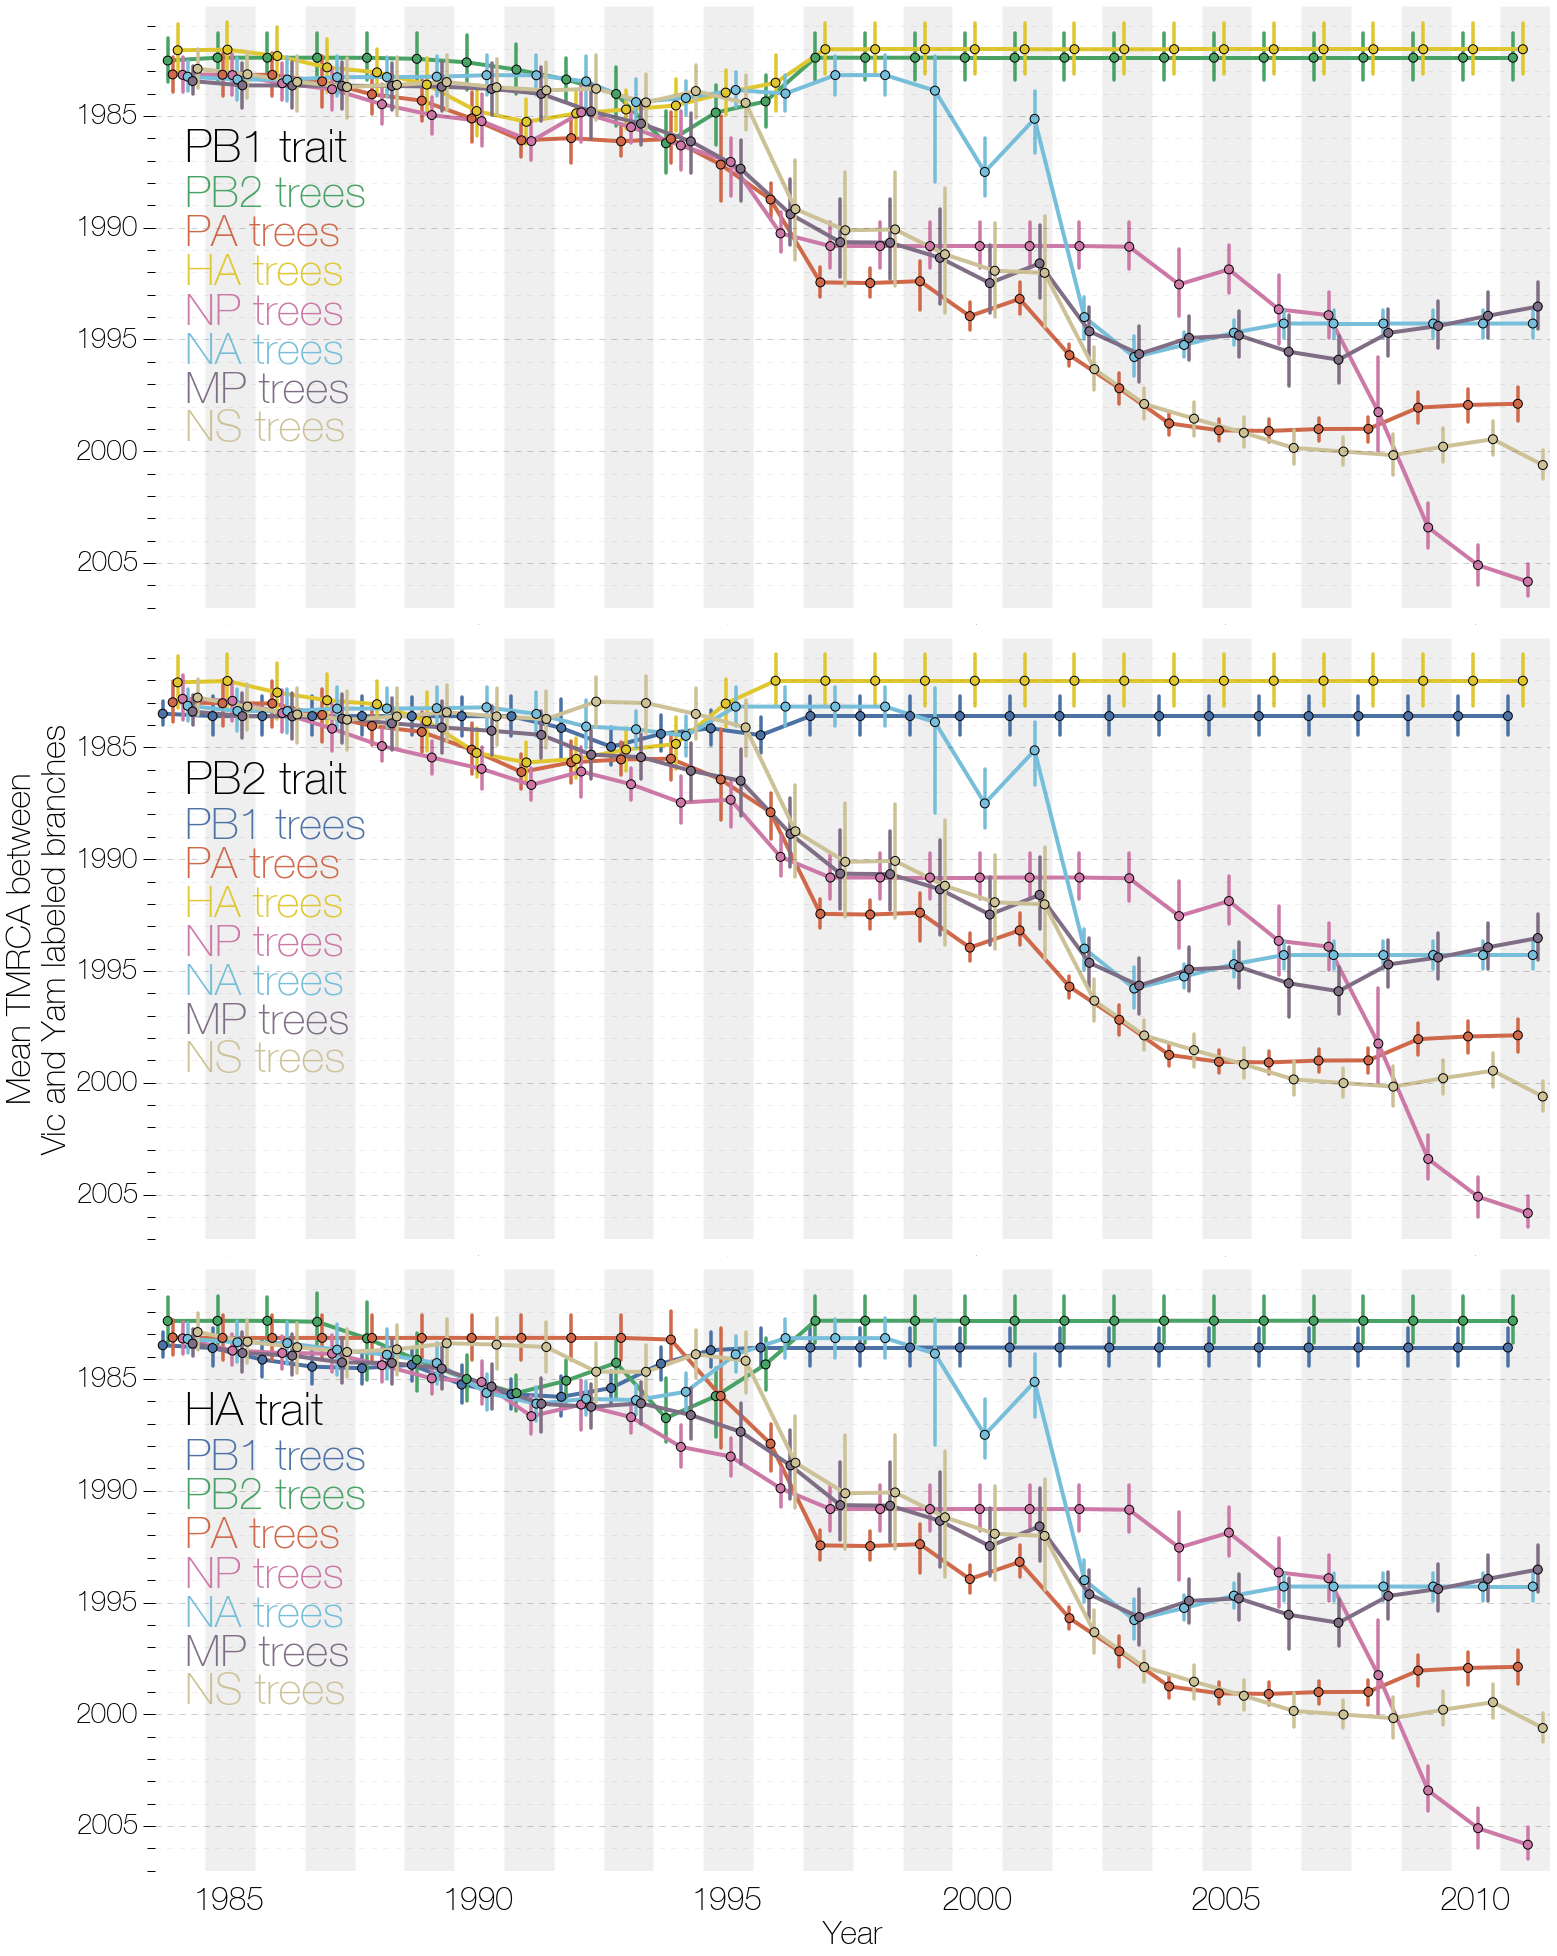
\includegraphics[width=0.95\textwidth]{figures/InfB_betweenDiversity.png}
	\caption{\textbf{Mean pairwise TMRCA between Vic and Yam branches under PB1, PB2 and HA label sets.}
PB1, PB2 and HA segment labels indicate that these segments show reciprocal preservation of diversity, which dates back to the split of Vic and Yam lineages.
All other segments show increasingly more recent TMRCAs between branches labelled as Vic and Yam in PB1, PB2 and HA label sets.
All vertical lines indicating uncertainty are 95\% highest posterior densities (HPDs).}
	\label{betweenDiversity}
\end{figure}

\subsection*{Railroad schematic plot of influenza B reassortment history}

\tbc{Are the observed rates of extinction / co-option fit with the effective population of the flu B population?  I.e. we generally get 10 years back to a common ancestor within a lineage / segment.  Can we think of the extinction of segments as an aspect of there existing a loosely panmictic flu B population for everything but PB1, PB2 and HA?}

We reconstructed reassortment events detectable by discrete traits.
Figure \ref{railroadPlot} focuses only on reassortments that have occured after 1990.
We identify 5 major reassortant genome constellations (given in order PB1-PB2-PA-HA-NP-NA-MP-NS) circulating 1992 -- 2011: B/Alaska/12/1996-like (YYYYYYYV), B/Nanchang/2/1997-like (VVYVYVYV), B/Iowa/03/2002-like (VVYVYYYV), B/California/NHRC0001/2006-like (VVYVYYYV) and B/Brisbane/33/2008-like (VVYVYYYV).
Figure \ref{railroadPlot} shows that reassorting segments appear to evolve with a considerable degree of autonomy.
For example, the NP lineage that entered a largely Victoria lineage derived genome and gave rise to the B/Nanchang/2/1997-like isolates continued circulating until 2010, even though other segments it reassorted with in 1995 -- 1996 (PA and MP) went extinct following the reassortments that led to B/Iowa/03/2002-like isolates.
A more extreme example is the NS segment, which in B/Iowa/03/2002-like isolates (and all subsequent Vic PB1-PB2-HA isolates) has been derived from Victoria lineage that had been associated with mostly Yam lineage derived B/Alaska/12/1996-like genomes for a number of years.

\begin{figure}
	\centering		
	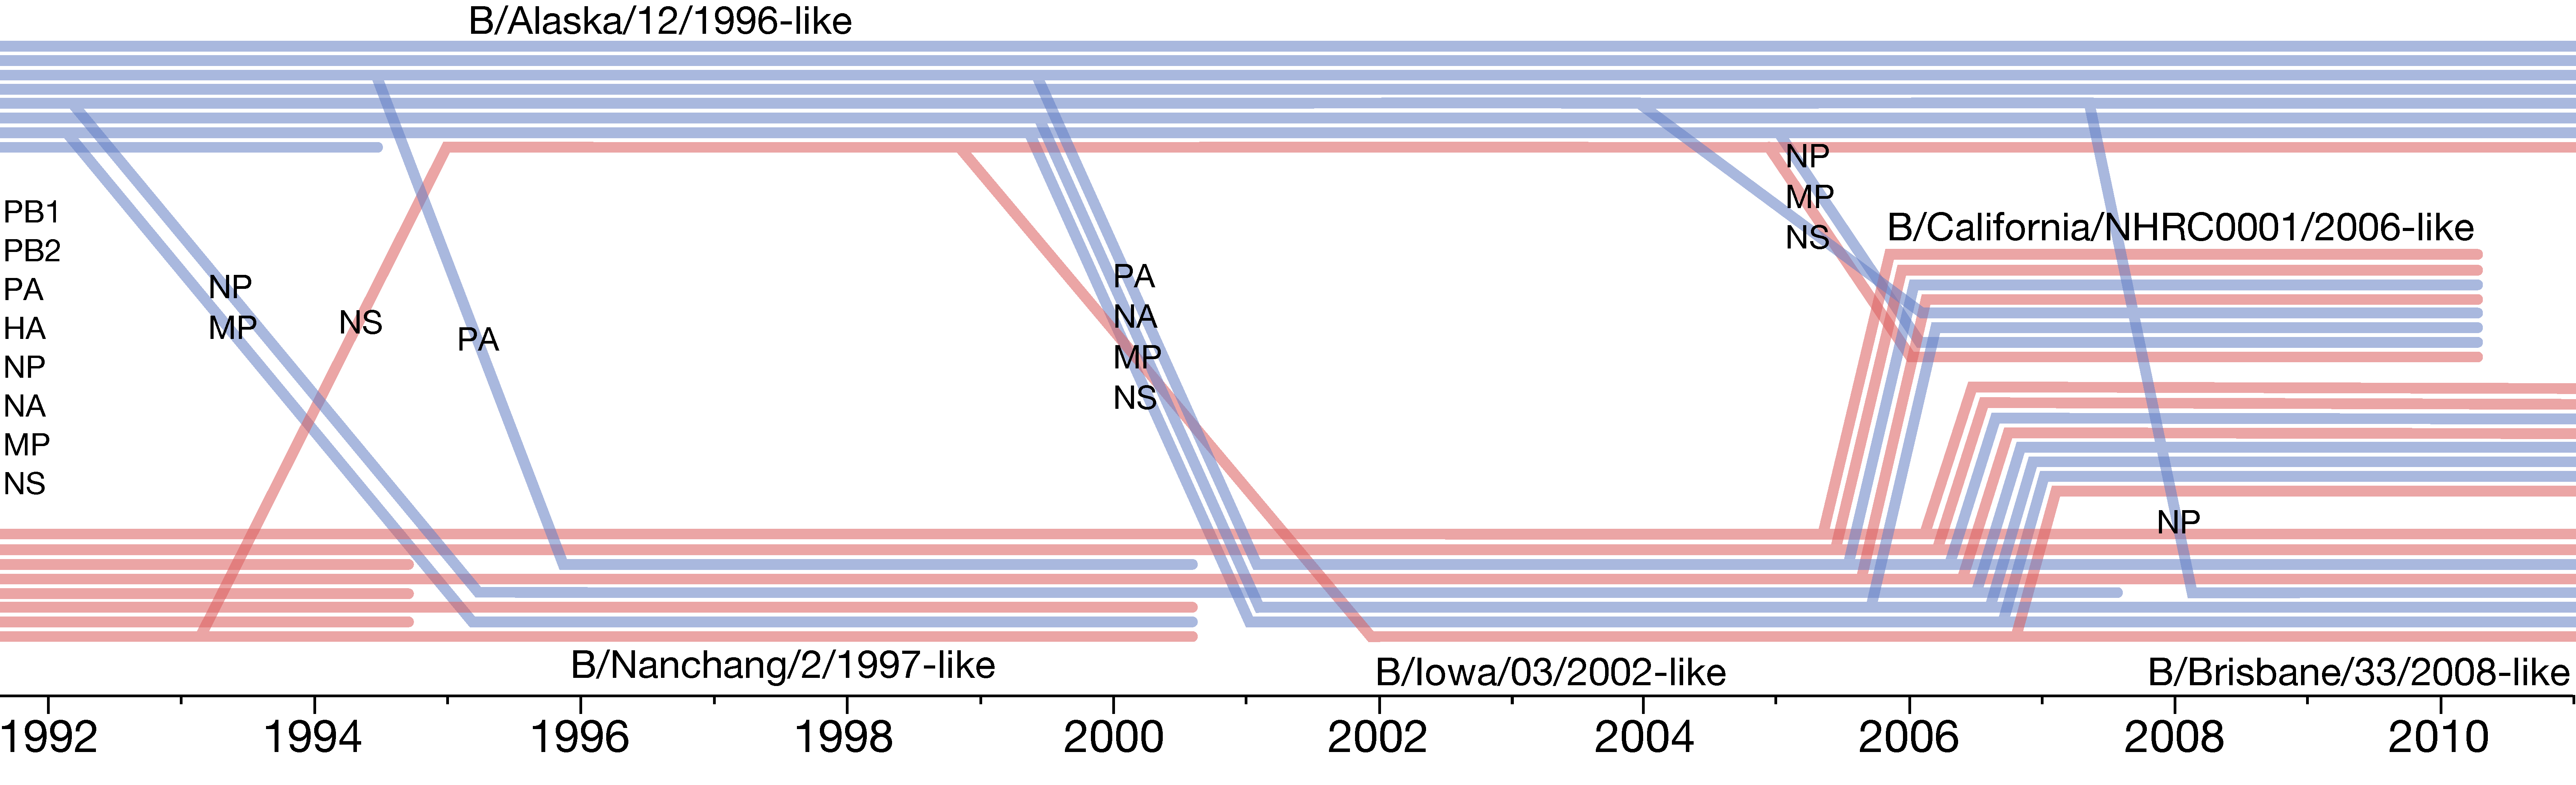
\includegraphics[width=0.95\textwidth]{figures/RailroadPlotDated.pdf}
	\caption{\textbf{Schematic plot of reconstructed reassortments between Victoria and Yamagata lineage segments of influenza B virus.}
Victoria and Yamagata lineage genomes are represented by 8 (red or blue, respectively) parallel lines.
Inter-lineage reassortment events are indicated by lines entering a different genome.
The angle of incoming lineages represents uncertainty in the timing of the event (mean date of the parent node and mean TMRCA of reassortant clades).
Lineage extinction dates are not shown accurately.}
	\label{railroadPlot}
\end{figure}


\subsection*{Numbers of reassortments are not significantly different between all segments, but reassortment distances can be}
Estimates of normalized SPR distances between pairs of segments (Figure \ref{SPRdistances}) show that there is no evidence of differences in reassortment rates between all segments, based on overlapping 95\% highest posterior density (HPD) intervals.


\begin{figure}
	\centering		
	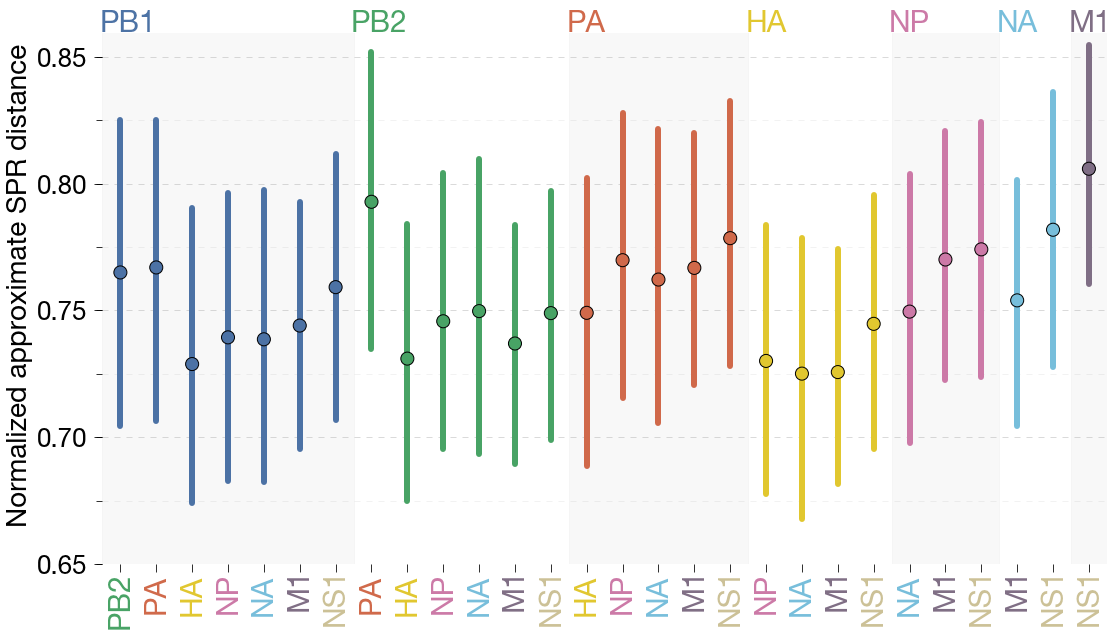
\includegraphics[width=0.95\textwidth]{figures/InfB_normalizedApproxSPR.png}
	\caption{\textbf{Normalized approximate SPR distances between pairs of segments.}
All vertical lines indicating uncertainty are 95\% highest posterior densities (HPDs).}
	\label{SPRdistances}
\end{figure}

Unlike normalized SPR distances normalized $\Delta$TMRCA estimates between some segments (Figure \ref{deltaTMRCA}) indicate that reassortment distance (as quantified by $\Delta$TMRCA) between some segments, namely PB1-PB2-HA (but also NA-M1 and PA-M1-NS1), are much more similar to $\Delta$TMRCA estimates between replicate trees.

\begin{figure}
	\centering		
	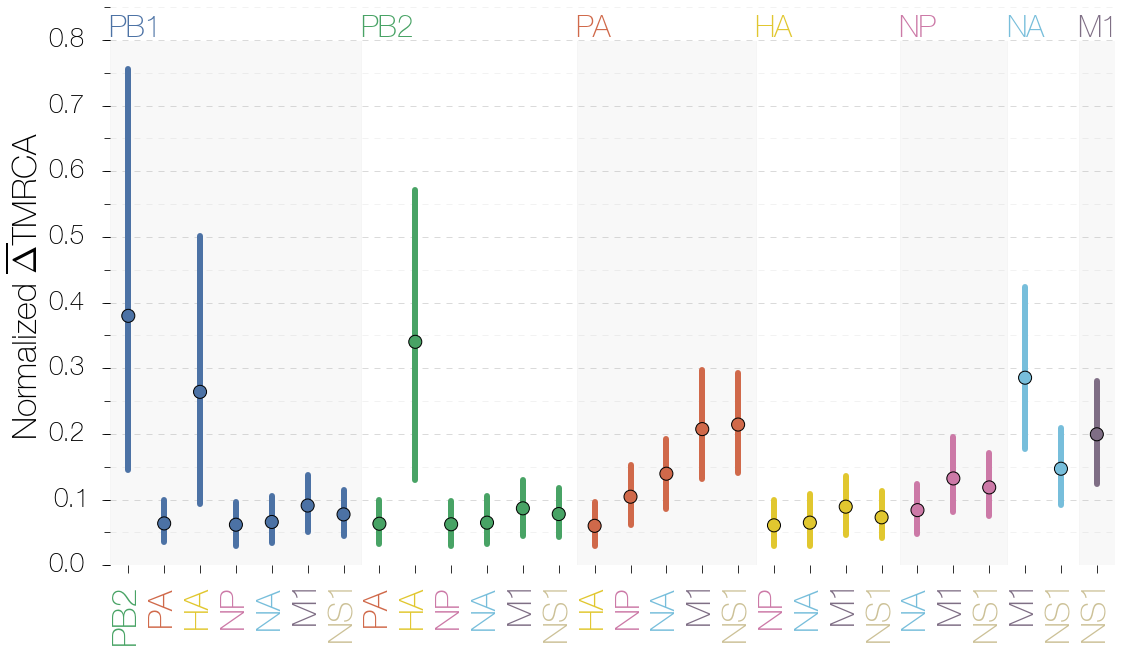
\includegraphics[width=0.95\textwidth]{figures/InfB_normalizedMuDeltaTMRCA.png}
	\caption{\textbf{Normalized mean $\Delta$TMRCA statistics between pairs of segments.}
All vertical lines indicating uncertainty are 95\% highest posterior densities (HPDs).}
	\label{deltaTMRCA}
\end{figure}


\subsection*{Linkage disequilibrium analysis confirms phylogenetic findings}
Linkage disequilibrium analyses (Figure \ref{segmentLD}) confirm our findings from phylogenetic analyses that PB1, PB2 and HA segments are linked.
We observe much higher mean $\chi^{2}_{df}$ between PB1, PB2 and HA amino acid sites than any other pair of proteins.
In some cases this value exceed the estimated LD of amino acid sites within the same protein (e.g. PB1 and HA).
Of the amino acid sites that exhibit high LD on PB1, PB2 and HA proteins, there are 5 sites on PB1, 8 on PB2 and 13 on HA proteins which form a network of sites exhibiting reciprocally high LD.
These sites define the split between Vic and Yam lineages within those segments.
In addition, there are sites on PB1, PB2 and HA proteins which also show high (albeit smaller) LD which correspond to sites which have undergone amino acid replacements some time after the Vic/Yam split.


\tbc{The 8x8 MDS analysis suggests that PB1-PB2-HA are the only segments with substantial coevolution.}

\subsection*{Amino acid sites with high LD between PB1, PB2 and HA}


We perform hierarchical clustering to identify clusters of sites which exhibit similar LD patterns across pairs of segments.


\begin{figure}[h]
	\centering	
	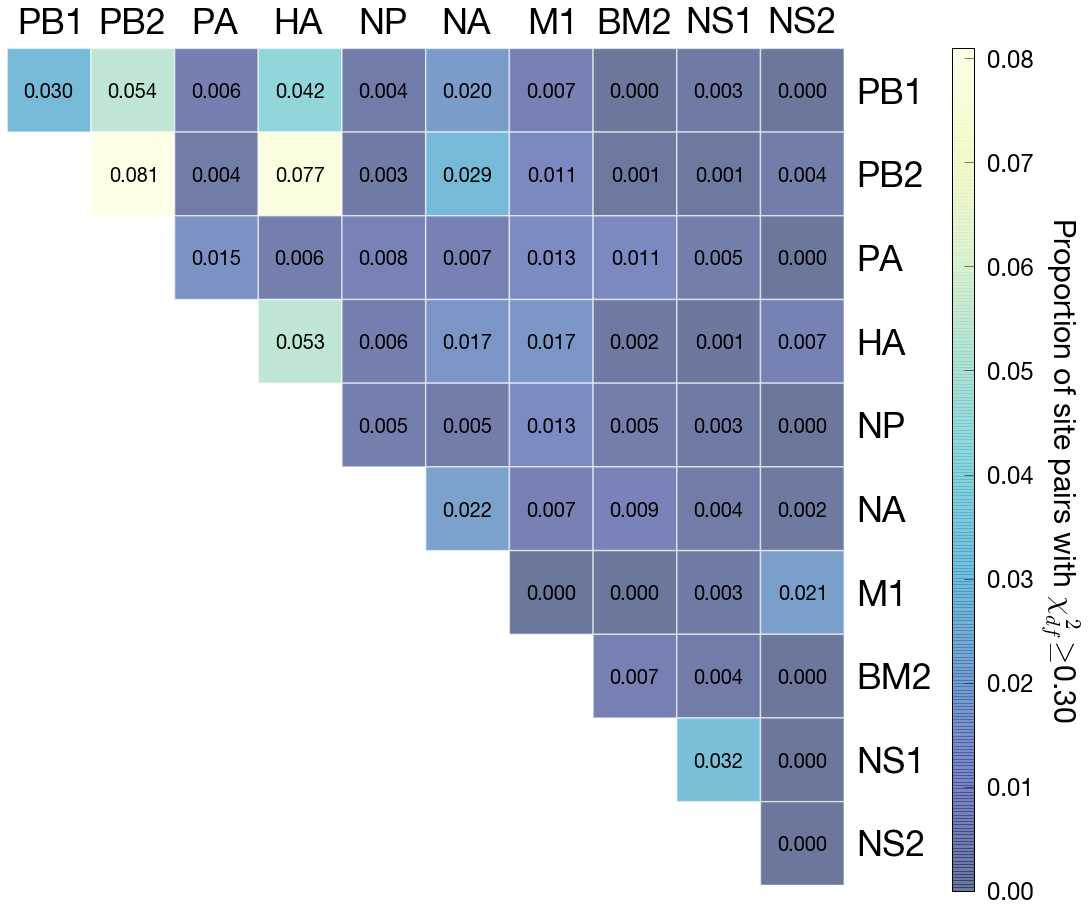
\includegraphics[width=0.75\textwidth]	{figures/InfB_segmentLD.png}
	\caption{\textbf{LD comparison between influenza B proteins.}
Comparison of linkage disequilibrium between amino acid sites on influenza B proteins.
Numbers on the heatmap are mean $\chi^{2}_{df}$ between pairs of proteins.}
	\label{segmentLD}
\end{figure}

(comment - will require a lot of fiddling to get the heatmaps displayed in a clear way)
\begin{figure}[h]
	\centering	
	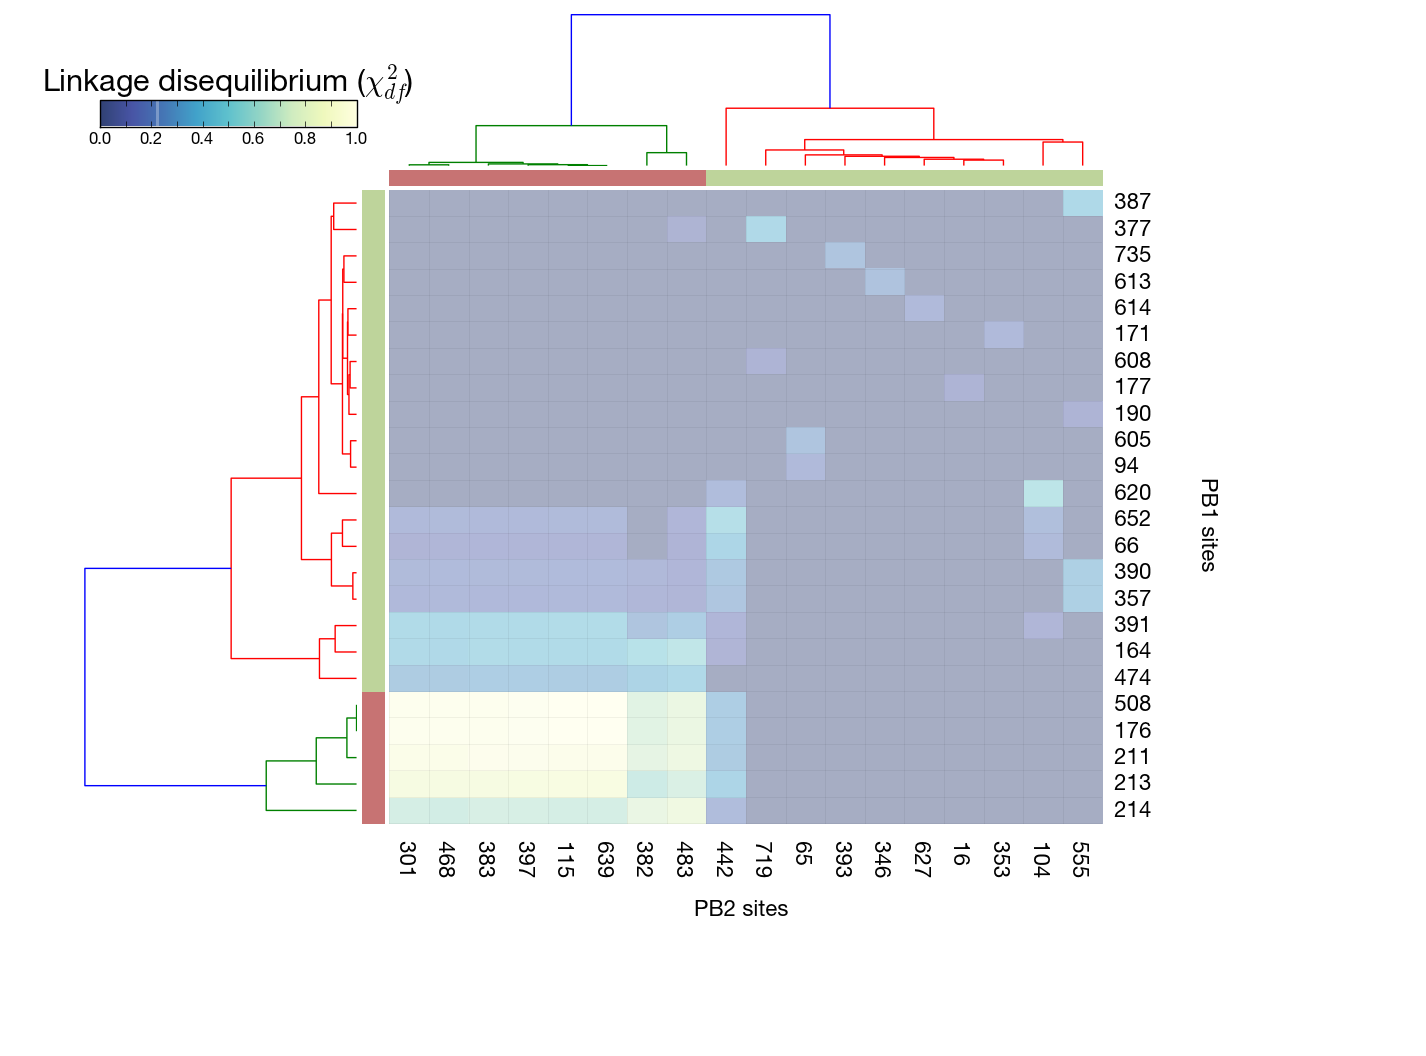
\includegraphics[width=0.65\textwidth]	{figures/Chi_PB1_PB2.png}
	\caption{\textbf{Hierarchical clustering of amino acid sites on PB1 and PB2 segments based on $\chi^{2}_{df}$ values.}}
	\label{ChiPB1PB2}
\end{figure}

\begin{figure}[h]
	\centering	
	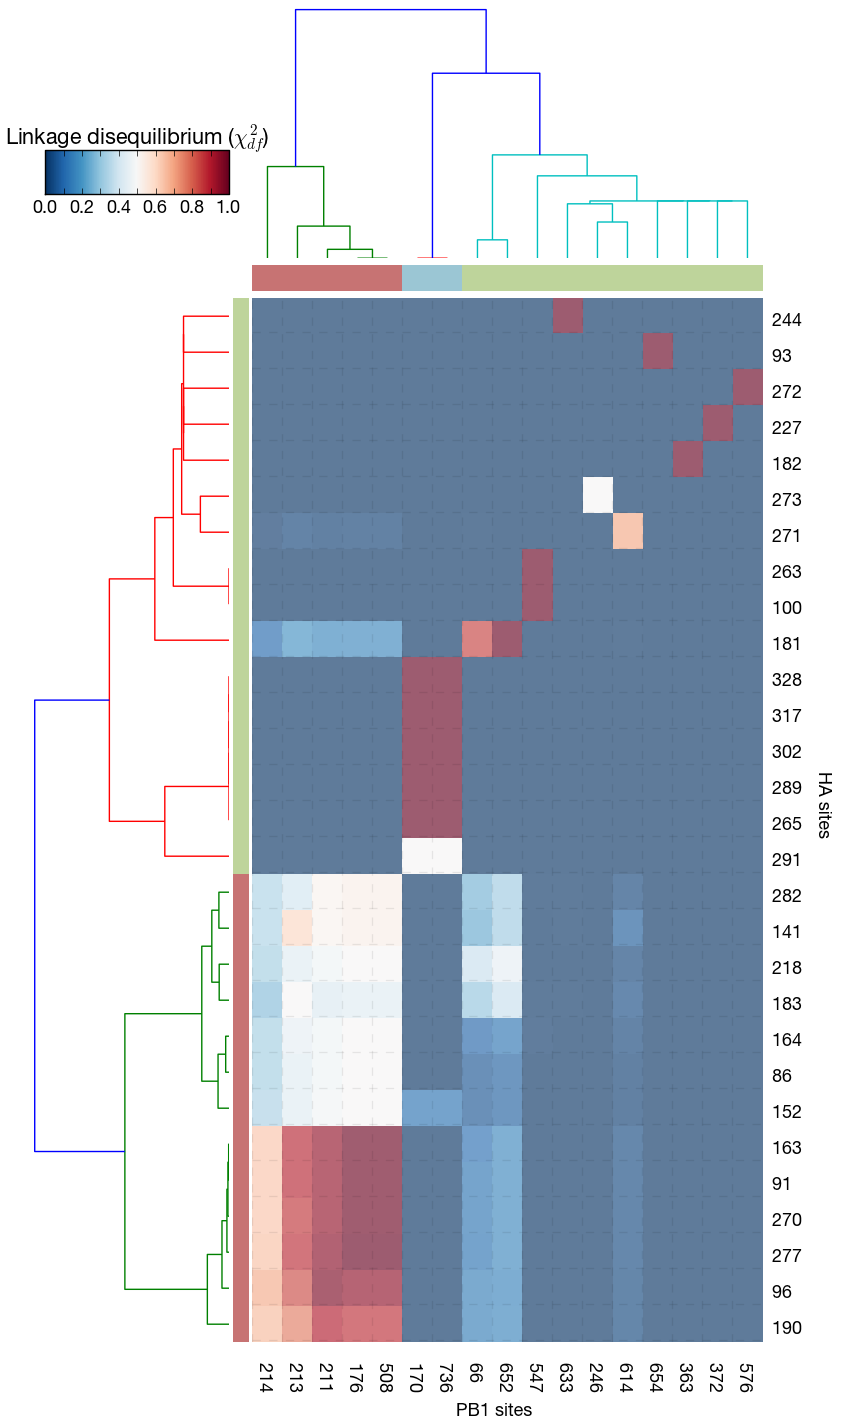
\includegraphics[width=0.65\textwidth]	{figures/Chi_PB1_HA.png}
	\caption{\textbf{Hierarchical clustering of amino acid sites on PB1 and HA segments based on $\chi^{2}_{df}$ values.}}
	\label{ChiPB1HA}
\end{figure}

\begin{figure}[h]
	\centering	
	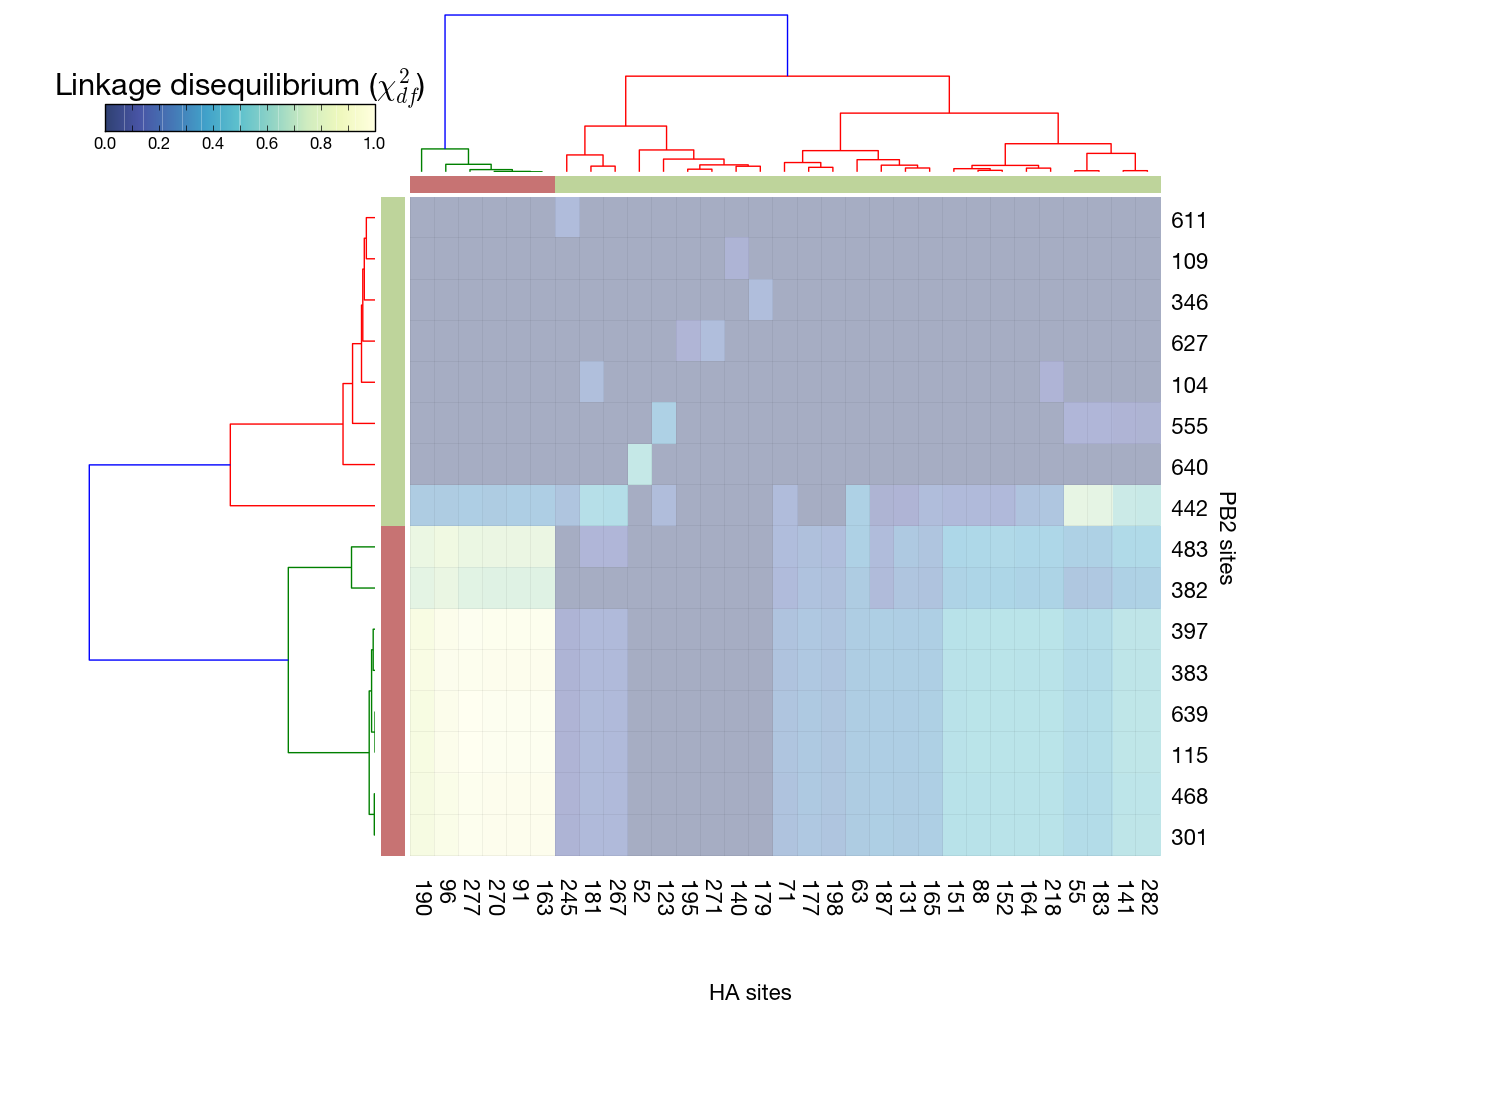
\includegraphics[width=0.65\textwidth]	{figures/Chi_PB2_HA.png}
	\caption{\textbf{Hierarchical clustering of amino acid sites on PB2 and HA segments based on $\chi^{2}_{df}$ values.}}
	\label{ChiPB2HA}
\end{figure}


\section*{Discussion}

\subsection*{Rehash streamlined version of results for people who don't read results sections.}
In this paper we have shown that PB1, PB2 and HA segments of influenza B viruses are the only ones that have maintained both a Vic and a Yam lineage (Figure \ref{LineageRatiosOverTime}).
Evidence suggests that this is a result of lack of reassortment between Vic and Yam lineages of these segments (Figure \ref{betweenDiversity}) which have evolved co-assorting amino acid sites detectable as high linkage disequilibrium (\ref{segmentLD}).
We propose that this pattern of non-reassortment is due to the action of selection and not simply biased reassortment.
Figures \ref{SPRdistance} and \ref{deltaTMRCA} show that despite all pairs of segments having the same reassortment frequency, PB1, PB2 and HA segments exhibit much lower reassortment `distances'.
In addition, most strains with mixed-lineage PB1-PB2-HA complexes occured in the early years of the Vic--Yam split, when the two lineages were much more similar at the nucleotide and amino acid levels.
The most recent lineage of influenza B viruses with mixed-lineage PB1-PB2-HA complexes (B/Waikato/6/2005-like) only circulated for 5 months before going extinct.
We suggest that the preservation of two PB1-PB2-HA complex lineages is similar to genomic speciation islands.
If both PB1-PB2-HA complex lineages continue circulating in humans we expect more segments to be recruited to the two complexes, resulting in eventual sympatric speciation of influenza B viruses. 
\tbc{Title is approximate.}

\subsection*{Limitations of current study}
The methods used in this paper have limited power to detect reassortments, since lineages have been fixed over time and thus all viruses eventually come to bear either Vic or Yam lineage PA, NP, NA, MP and NS segments with the exception of PB1, PB2 and HA segments.
We can also only detect reassortment events where a lineage has switched from Vic to Yam or \textit{vice versa}, but not when a lineage has switched from a Yam lineage to another Yam lineage, which has occurred in the past (e.g. the reassortment events giving rise to B/California/NHRC0001/2006-like and B/Brisbane/33/2008-like viruses in Figure \ref{railroadPlot}, which involved a Vic lineage PB1-PB2-HA complex reassorting with NP of Yamagata lineage is only visible in the NP tree, since all viruses in our dataset from 1995 onwards, including Vic PB1-PB2-HA complex-bearing ones, already had a Yamagata lineage-derived NP).
However, this study focuses on PB1, PB2 and HA segments, all of which have survived as two lineages up to this day and thus are more informative for inferring reassortments.

\subsection*{PB1-PB2-HA co-adaptation has evolved over time}
Our findings suggest that PB1, PB2 and HA segments of Vic and Yam lineages represent co-adapted co-reassorting segment complexes.
Previous studies have suggested similarities between the evolution of PB1, PB2 and HA segments of influenza B viruses \cite{hiromoto2000,lindstrom1999}, based on topology similarities between phylogenetic trees of the three segments, albeit the trees used contained limited numbers of sequences sampled somewhat close in time to the split of Victoria and Yamagata lineages.
Despite the apparent similarities between PB1, PB2 and HA trees, we have detected at least 4 genome constellations having mixed-lineage PB1-PB2-HA, 3 of which were sampled early in the first decade of the split between Vic and Yam lineages, when, presumably, Vic and Yam lineages of PB1, PB2 and HA segments were still similar at the amino acid level to produce viable, though presumably unfit, influenza B viruses.
The fourth genome constellation having mixed-lineage PB1-PB2-HA complex was isolated in Australia and New Zealand in 2005 over a 5 month period and have not been detected since.

Our results also suggested that all segments have spent very little evolutionary time with the 3 mixed-lineage PB1-PB2-HA constellations, compared to either entirely Yam PB1-PB2-HA or entirely Vic PB1-PB2-HA bearing viruses.
We interpret lack of reassortment within the PB1-PB2-HA complex across the Vic--Yam lineage boundary in recent times as evidence of a considerable degree of co-dependence within the Vic and Yam PB1-PB2-HA lineages, whereby recent reassortants bearing mixed-lineage PB1-PB2-HA complexes are inviable or unsampled by surveillance due to being outcompeted by viruses with pure-lineage PB1-PB2-HA complexes.

We have identified amino acid sites which exhibit a high degree of linkage disequilibrium between PB1, PB2 and HA segments.
Sites with high LD on PB1, PB2 and HA segments could be interpreted as either sites which have drifted apart due to lack of reassortment between the three segments or as sites which prevent the cooperation of the three proteins at the molecular level and thus prevent inter-lineage PB1-PB2-HA reassortants from having comparable fitness to viruses with `pure' lineage PB1-PB2-HA complexes.

None of the sites we have identified on PB1 and PB2 proteins fall within the previously described regions that form the contacts between the two polymerase subunits \cite{sugiyama2009}.

Sites 211, 213 and 214 on the PB1 protein are very close to each other and the stretch of sequence around these residues contains many positively charged amino acids (lysine and arginine).
Multiple nuclear localization signals (NLSs) are predicted to occur around this region and sites 211, 213 and 214 are either predicted to be near the end of a mono-partite NLS or the beginning of a bi-partite NLS.
Previous research \cite{nath1990} suggests that in the influenza A PB1 protein residue 211 (homologous to influenza B PB1 residue 211) is the last residue of a bi-partite NLS.
Almost all Yamagata lineage isolates possess arginine (R) residue at PB1 positions 211 and 214 and a serine (S) residue at position 213, whereas Victoria lineage isolates have lysine (K) at positions 211 and 214 and threonine (T) at position 213.
It remains to be seen whether these sites significantly affect the nuclear import efficiency of the PB1 protein of either lineage.
Though the PB1 protein is known to accumulate in the nucleus on its own, efficient import into the nucleus requires the presence of the PA protein \cite{fodor2004}.
Similarly, sites 382 and 397 on the PB2 protein are close to residues 377, 406 and 408 which are homologous to sites in influenza A that are responsible for mRNA cap-binding \cite{guilligay2008}.
Again, we cannot determine whether this finding is significant or not.


\subsection*{All segments reassort equally but some are more equal than others}
The 95\% HPD intervals of normalized approximate SPR distances between pairs of segments (Figure \ref{SPRdistances}) overlap, suggesting there is no evidence of differences in the numbers of reassortments (or reassortment rate given as number of SPR moves per tree, data not shown) between all segments.
There is reason to suspect that our SPR distance analysis simply lacks power.
We used an approximation of the true SPR distances and SPR distances themselves could only approximate (and underestimate) the actual numbers of reassortments.
However, exact SPR distances could be estimated for a limited number of segment pairs (PB1--PB2 and PB1--HA) and analyses indicate that after normalization exact and approximate SPR distances are not significantly different (supplementary figure of exact-approximate SPR distance differences and/or correlations of the two?). 

Significant differences between pairs of segments can be found when considering `reassortment distance'.
Our estimates suggest that tips in PB1, PB2 and HA trees have similar TMRCAs (Figure \ref{deltaTMRCA}), suggesting that reassortments between the three rarely bring together lineages that have been evolving separately for prolonged periods of time.
We cannot determine whether this effect is specifically due to non-reassortment of Vic and Yam PB1-PB2-HA lineages or a generic property of these three segments.
In addition, we see evidence of this in MP and NA trees (comment - get references for MP-NA association in fluA, otherwise put down as personal communication or commonly held suspicion).


\subsection*{Potential causes of co-dependence between PB1-PB2-HA}
Previous studies have investigated possible co-dependence patterns between segments of influenza B viruses, by focusing on segments which would be expected to be co-adapted, e.g. PB1-PB2-PA and HA-NA \cite{mccullers2004}.
Though it would be easy to explain co-adaptation between the aforementioned segments by referring to their functional roles (e.g. PB1-PB2-PA form the polymerase heterotrimer and HA-NA have antagonistic activities), our findings suggest a counter-intuitive relationship between PB1, PB2 and HA segments.

It is clear that PB1-PB2-HA segments of Vic and Yam lineages do not preferentially reassort together: there have been at least 4 sampled mixed-lineage PB1-PB2-HA complex constellations (which did not become fixed in the population), our estimates of the number of reassortments do not differ significantly between all segments (Figure \ref{SPRdistances} and recent evidence suggests that, at least in influenza A, reassortment between segments differing by a single synonymous difference is highly efficient \cite{marshall2013}.
In the absence of clear functional explanations for why PB1, PB2 and HA should be co-adapted we suggest several alternatives.

It is perhaps easiest to explain co-dependence between PB1 and PB2 segments based on their functions as part of the influenza RNA-dependent RNA polymerase (RdRp) heterotrimer.
Indeed, trees of PB1 and PB2 segments exhibit high similarity in tip--tip TMRCAs (Figure \ref{deltaTMRCA}), suggesting highly similar trees.
In addition, PB1--PB2 reassortants are the rarest and least persistent amongst mixed-lineage PB1-PB2-HA strains and have not been isolated since 1996.

Explaining the co-dependence between PB1+2 and HA segments is more difficult.

Many studies have noted a possible link between the HA, NA and PB1 segments of influenza A viruses \cite{bergeron2010,fulvini2011}.
Early influenza A vaccines were derived by infecting chicken eggs with an egg-adapted strain and a seasonal human isolate in the presence of antisera raised against the HA and NA proteins of the egg-adapted strain, thus selecting for reassortants which were egg-adapted (\textit{i.e.} had internal segments derived from the egg-adapted strain) but possessed the HA and NA segments of the seasonal strain.
However, in addition to producing reassortants with HA-NA derived from the seasonal strain, as intended, the second most frequent class of reassortants produced using this methods were those with PB1, HA and NA derived from seasonal strains \cite{bergeron2010,fulvini2011}.

Recent experiments have suggested that the presence or absence of a `foreign' PB1 segment can have dramatic effects on HA concentration on the surface of virions and total virion production \cite{cobbin2013}.
Additional evidence for a relationship between PB1 and HA segments in influenza A viruses is given by previous influenza pandemics, which were caused by avian-human influenza A virus reassortants.
It has been established that at least for the 1957 and the 1968 influenza pandemics, caused by A/H2N2 and A/H3N2 subtypes, respectively, the viruses responsible were reassortants possessing PB1 and HA segments (and in the case of A/H2N2, NA as well) derived from avian influenza A viruses \cite{kawaoka1989}.
However, there have also been reassortant influenza viruses circulating for prolonged periods of time in humans that did have disparate PB1 and HA segments, \textit{e.g.} H1N2 outbreaks in 2001 \cite{gregory2002} and H1N1/09 in 2009 \cite{smith2009}.


Another possibility is the action of balancing selection in preserving the diversity in one segment, whilst the other segments hitchhike along.
A good candidate for this would be HA, as it is now the sole bearer of antigenic diversity within the influenza B population (the Vic lineage NA segment having gone extinct in 2002), until the Yam lineage NA segment under Vic PB1-PB2-HA recovers sufficient antigenic diversity.
Previous research has found that avian influenza A virus HA and NA segments, which are the primary vehicles of antigenicity, exhibit vast diversity when compared to `internal segments', which show much more recent TMRCAs and less variability at the amino acid level \cite{chen2006,obenauer2006}.
It is also possible that Vic and Yam lineages of PB1, PB2 and HA segments have simply drifted away from each other, without any one segment being the driver of diversity preservation in PB1, PB2 and HA segments.
This process, termed mutation-driven co-evolution \cite{presgraves2010}, has been suggested to be the cause of hybrid dysfunction in \textit{Saccharomyces} hybrids \cite{lee2008}.

Though it is possible that PB1 and PB2 segments are co-adapted and the HA segment is simply hitchhiking along stochastically, we find it unlikely given that B/Waikato/6/2005-like strains, the most recent isolates with a mixed-lineage PB1-PB2-HA complex, circulated for a limited amount of time within a limited geographic area, suggesting that this particular lineage was outcompeted by influenza B strains with `pure' PB1-PB2-HA complexes.

\subsection*{The future of influenza B viruses}
We see two potential paths of evolution for influenza B viruses.
More segments could be recruited into co-adapted segment complexes (PB1, PB2 and HA segments having started this first, akin to genomic speciation islands), as part of a speciation process, until all circulating influenza B viruses possess genomes with segments firmly associated with either the Vic or Yam lineage PB1-PB2-HA complex which could be referred to as belonging to either `new Victoria' or `new Yamagata' lineages.

This may seem to be the case in Figure \ref{tmrcaOT} where the NP segment, exhibiting the fourth oldest TMRCA by 2011, looks like it might begin co-evolving with the PB1-PB2-HA complexes. 
However, the continuous measure of diversity between Vic and Yam lineages of PB1, PB2 and HA segments in Figure \ref{betweenDiversity} show that the NP segment is skewed towards very recent TMRCAs, suggesting that a large number of recent isolates are products of recent reassortment between the NP segment and PB1-PB2-HA complexes.
In fact, this is due to viruses possessing B/Brisbane/33/2008-like genome constellations, which comprise a large part of recently isolated influenza B virus strains (Figure \ref{railroadPlot}).
The other alternative is continued reassortment of all non-PB1-PB2-HA segments between Vic and Yam PB1-PB2-HA complexes, or even extinction of one or the other lineage of the PB1-PB2-HA complex.

Given the relatively recent explosion of sequence data available for influenza B, it is difficult to say whether such two-lineage dynamics have not occurred in the history of influenza B viruses.
If the influenza B population is on its way to speciation we expect that over time inter-lineage reassortment frequency should decrease, as more and more segment lineages would be recruited into co-adapted segment complexes.

On the other hand, influenza B viruses might continue co-circulating as two PB1-PB2-HA lineages exchanging non-PB1-PB2-HA segments, with reassortment frequency being roughly constant.
Seeing how rarely influenza B viruses reassort across the Vic-Yam lineage boundary, the timescale for finding out which of the aforementioned scenarios, if any, are under way, is impractical at best.

\subsection*{Predictions}
Using previously developed plasmid systems \cite{hoffmann2002} it would be possible to create artificial reassortants, combining Vic and Yam lineages of PB1, PB2 and HA segments into mixed-lineage PB1-PB2-HA complexes.
We predict that artificially produced viruses with mixed-lineage PB1-PB2-HA complexes will have reduced fitness when compared to viruses with pure-lineage (\textit{i.e.} entirely Vic or entirely Yam) PB1-PB2-HA complexes.
In addition, we expect the relationship between Vic and Yam lineage PB1, PB2 and HA segments to be dependent on date of segment isolation, as viruses with mixed-lineage PB1-PB2-HA complexes isolated earlier should perform better than viruses with PB1-PB2-HA segments isolated more recently.

Given the existence of B/Waikato/6/2005-like viruses and the rarity of PB1-PB2 reassortants we expect that artificially produced PB1-PB2 reassortants would be much less fit than either PB1+2-HA reassortants.

However, we also see that epistatic effects might interfere with fitness measurements, if for example non-PB1-PB2-HA segments are also temporally mismatched.
Ideally, the co-adaptation would be easier to understand by referring to the structures of PB1 and PB2 proteins, as the link between these would be intuitive.
We have identified amino acid sites which are linked between PB1, PB2 and HA proteins of Victoria and Yamagata lineages, but we find very few sites on PB1 and PB2 proteins that fall within the regions that form contacts within the influenza B polymerase heterotrimer, suggesting more subtle roles for sites we have identified.

\subsection*{Implications for influenza B virus control and prevention}
It is our hope that understanding the mechanism(s) underlying the links between Vic and Yam lineage PB1-PB2-HA complexes might suggest a more varied approach to both influenza B surveillance and control.
For one, our findings suggest that viruses bearing mixed-lineage PB1-PB2-HA complexes, if unveiled by surveillance, are unlikely to contribute to future influenza B evolution.
Similarly, in the absence of sequence data, it should be possible to predict the lineage of PB1, PB2 and HA segments of influenza B viruses by sequencing only one of those segments.

It remains to be seen whether equivalent or similar links exist between segments of influenza A viruses, which present a much greater threat to human health worldwide than influenza B viruses.
By discovering the underlying mechanism by which PB1, PB2 and HA are co-adapted might reveal potential targets for new classes of antiviral drugs.

\section*{Conclusions}
In this study we have investigated the patterns of reassortment amongst two influenza B virus segment lineages and found preserved diversity and consistent co-reassortment of 3 segments: PB1, PB2 and HA.
Our findings reveal that Vic and Yam lineages of PB1, PB2 and HA segments co-associate amongst themselves with segments of their own lineage, thus resulting in an entirely Vic-lineage-derived PB1-PB2-HA segment complex and an entirely Yam-lineage-derived PB1-PB2-HA segment complex that co-circulate within the influenza B virus population, occasionally exchanging non-PB1-PB2-HA segments.
Though we detect strains with mixed-lineage PB1-PB2-HA complexes, we find that they have performed poorly and have circulated for short amounts of evolutionary time when compared to viruses with `pure' lineage PB1-PB2-HA complexes.

We argue that this is evidence for a selectively maintained relationship between PB1-PB2-HA complex of Vic and Yam lineages and not due to biased reassortment.
Given sufficient time we expect the two PB1-PB2-HA complexes to recruit the rest of the genomic segments into co-adapted and co-reassorting segment complexes eventually resulting in sympatric speciation of influenza B viruses.


%\begin{figure}[h]
%	\centering		
%	\includegraphics[width=0.95\textwidth]{figures/InfB_TMRCAOverTime}
%	\caption{\textbf{Provisional TMRCA over time plot.}}
%\end{figure}


\bibliographystyle{pnas}
\bibliography{fluB}
\end{document}
